\makeatletter
\pgfkeys{/pgf/.cd,
  parallelepiped offset x/.initial=2mm,
  parallelepiped offset y/.initial=2mm
}
\pgfdeclareshape{parallelepiped}
{
  \inheritsavedanchors[from=rectangle] % this is nearly a rectangle
  \inheritanchorborder[from=rectangle]
  \inheritanchor[from=rectangle]{north}
  \inheritanchor[from=rectangle]{north west}
  \inheritanchor[from=rectangle]{north east}
  \inheritanchor[from=rectangle]{center}
  \inheritanchor[from=rectangle]{west}
  \inheritanchor[from=rectangle]{east}
  \inheritanchor[from=rectangle]{mid}
  \inheritanchor[from=rectangle]{mid west}
  \inheritanchor[from=rectangle]{mid east}
  \inheritanchor[from=rectangle]{base}
  \inheritanchor[from=rectangle]{base west}
  \inheritanchor[from=rectangle]{base east}
  \inheritanchor[from=rectangle]{south}
  \inheritanchor[from=rectangle]{south west}
  \inheritanchor[from=rectangle]{south east}
  \backgroundpath{
    % store lower right in xa/ya and upper right in xb/yb
    \southwest \pgf@xa=\pgf@x \pgf@ya=\pgf@y
    \northeast \pgf@xb=\pgf@x \pgf@yb=\pgf@y
    \pgfmathsetlength\pgfutil@tempdima{\pgfkeysvalueof{/pgf/parallelepiped
offset x}}
    \pgfmathsetlength\pgfutil@tempdimb{\pgfkeysvalueof{/pgf/parallelepiped
offset y}}
    \def\ppd@offset{\pgfpoint{\pgfutil@tempdima}{\pgfutil@tempdimb}}
    \pgfpathmoveto{\pgfqpoint{\pgf@xa}{\pgf@ya}}
    \pgfpathlineto{\pgfqpoint{\pgf@xb}{\pgf@ya}}
    \pgfpathlineto{\pgfqpoint{\pgf@xb}{\pgf@yb}}
    \pgfpathlineto{\pgfqpoint{\pgf@xa}{\pgf@yb}}
    \pgfpathclose
    \pgfpathmoveto{\pgfqpoint{\pgf@xb}{\pgf@ya}}
    \pgfpathlineto{\pgfpointadd{\pgfpoint{\pgf@xb}{\pgf@ya}}{\ppd@offset}}
    \pgfpathlineto{\pgfpointadd{\pgfpoint{\pgf@xb}{\pgf@yb}}{\ppd@offset}}
    \pgfpathlineto{\pgfpointadd{\pgfpoint{\pgf@xa}{\pgf@yb}}{\ppd@offset}}
    \pgfpathlineto{\pgfqpoint{\pgf@xa}{\pgf@yb}}
    \pgfpathmoveto{\pgfqpoint{\pgf@xb}{\pgf@yb}}
    \pgfpathlineto{\pgfpointadd{\pgfpoint{\pgf@xb}{\pgf@yb}}{\ppd@offset}}
  }
}
\makeatother

\ifx\du\undefined
  \newlength{\du}
\fi
\setlength{\du}{1.5\unitlength}
\ifx\spacing\undefined
  \newlength{\spacing}
\fi
\setlength{\spacing}{30\unitlength}
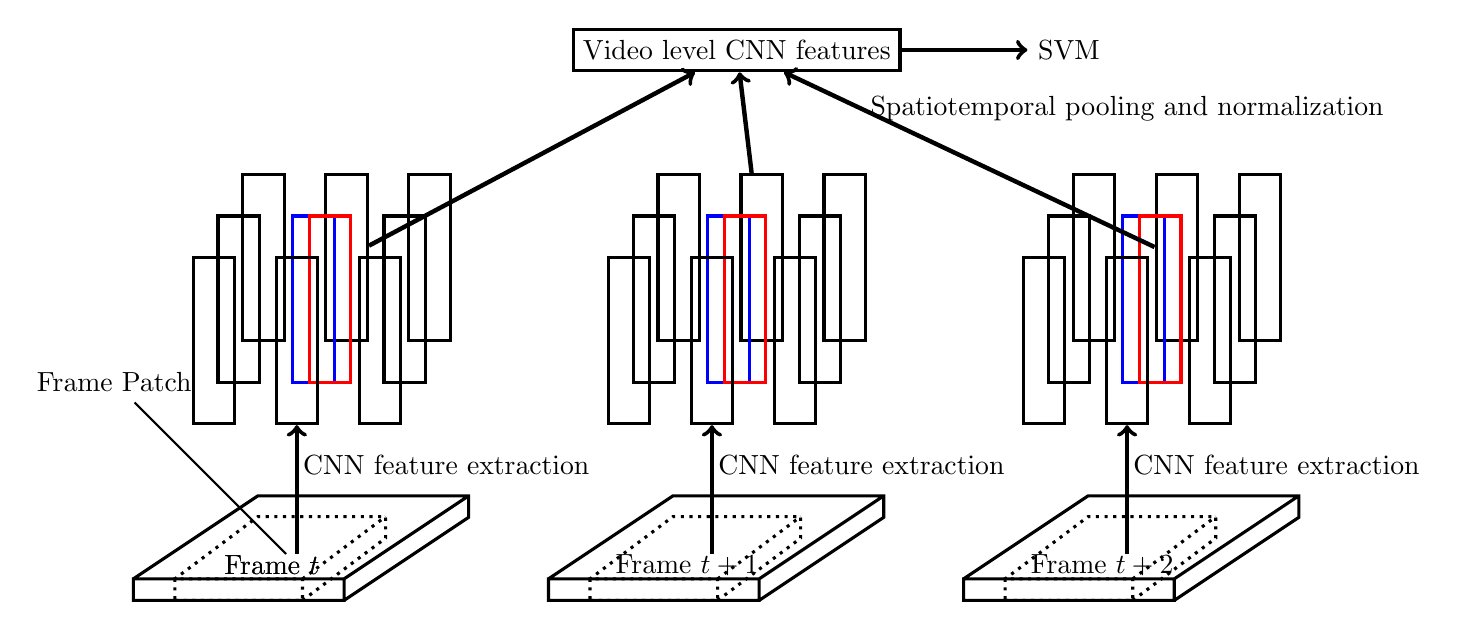
\begin{tikzpicture}
\pgfsetlinewidth{0.7500\du}
\pgfsetmiterjoin
\pgfsetbuttcap

\node[parallelepiped,draw=black,
  minimum width=50\du,minimum height=\du,
  parallelepiped offset x=30\du,
  parallelepiped offset y=20\du] (1a) at (0, -\spacing) {};
  \node[anchor=center] at (0.4\spacing, -0.7\spacing){Frame $t$};

\node[parallelepiped,draw=black, dotted,
  minimum width=30\du,minimum height=\du,
  parallelepiped offset x=20\du,
  parallelepiped offset y=15\du] (2a) at (0, -\spacing) {};

\node[anchor=center] at (0.4\spacing, -0.7\spacing){Frame $t$};



\node[parallelepiped,draw=black,
  minimum width=50\du,minimum height=\du,
  parallelepiped offset x=30\du,
  parallelepiped offset y=20\du] (1b) at (5\spacing, -\spacing) {};
  \node[anchor=center] at (5.4\spacing, -0.7\spacing){Frame $t+1$};

\node[parallelepiped,draw=black, dotted,
  minimum width=30\du,minimum height=\du,
  parallelepiped offset x=20\du,
  parallelepiped offset y=15\du] (2b) at (5\spacing, -\spacing) {};

\node[parallelepiped,draw=black,
  minimum width=50\du,minimum height=\du,
  parallelepiped offset x=30\du,
  parallelepiped offset y=20\du] (1c) at (10\spacing, -\spacing) {};
  \node[anchor=center] at (10.4\spacing, -0.7\spacing){Frame $t+2$};

\node[parallelepiped,draw=black, dotted,
  minimum width=30\du,minimum height=\du,
  parallelepiped offset x=20\du,
  parallelepiped offset y=15\du] (2c) at (10\spacing, -\spacing) {};

\node[rectangle, draw=black, minimum width=10\du, minimum height=40\du] (f1) at (0.3\spacing, 3.0\spacing) {};
\node[rectangle, draw=black, minimum width=10\du, minimum height=40\du] (f2) at (1.3\spacing, 3.0\spacing) {};
\node[rectangle, draw=black, minimum width=10\du, minimum height=40\du] (f3) at (2.3\spacing, 3.0\spacing) {};

\node[rectangle, draw=black, minimum width=10\du, minimum height=40\du] (f4) at (0\spacing, 2.5\spacing) {};
\node[rectangle, draw=black, minimum width=10\du, minimum height=40\du, color=blue] (f5) at (0.9\spacing, 2.5\spacing) {};
\node[rectangle, draw=black, minimum width=10\du, minimum height=40\du, color=red] (f10) at (1.1\spacing, 2.5\spacing) {};
\node[rectangle, draw=black, minimum width=10\du, minimum height=40\du] (f6) at (2\spacing, 2.5\spacing) {};

\node[rectangle, draw=black, minimum width=10\du, minimum height=40\du] (f7) at (-0.3\spacing, 2.0\spacing) {};
\node[rectangle, draw=black, minimum width=10\du, minimum height=40\du] (f8) at (0.7\spacing, 2.0\spacing) {};
\node[rectangle, draw=black, minimum width=10\du, minimum height=40\du] (f9) at (1.7\spacing, 2.0\spacing) {};


\node[rectangle, draw=black, minimum width=10\du, minimum height=40\du] (g1) at (5.3\spacing, 3.0\spacing) {};
\node[rectangle, draw=black, minimum width=10\du, minimum height=40\du] (g2) at (6.3\spacing, 3.0\spacing) {};
\node[rectangle, draw=black, minimum width=10\du, minimum height=40\du] (g3) at (7.3\spacing, 3.0\spacing) {};

\node[rectangle, draw=black, minimum width=10\du, minimum height=40\du] (g4) at (5\spacing, 2.5\spacing) {};
\node[rectangle, draw=black, minimum width=10\du, minimum height=40\du, color=blue] (g5) at (5.9\spacing, 2.5\spacing) {};
\node[rectangle, draw=black, minimum width=10\du, minimum height=40\du, color=red] (g10) at (6.1\spacing, 2.5\spacing) {};
\node[rectangle, draw=black, minimum width=10\du, minimum height=40\du] (g6) at (7\spacing, 2.5\spacing) {};

\node[rectangle, draw=black, minimum width=10\du, minimum height=40\du] (g7) at (4.7\spacing, 2.0\spacing) {};
\node[rectangle, draw=black, minimum width=10\du, minimum height=40\du] (g8) at (5.7\spacing, 2.0\spacing) {};
\node[rectangle, draw=black, minimum width=10\du, minimum height=40\du] (g9) at (6.7\spacing, 2.0\spacing) {};


\node[rectangle, draw=black, minimum width=10\du, minimum height=40\du] (h1) at (10.3\spacing, 3.0\spacing) {};
\node[rectangle, draw=black, minimum width=10\du, minimum height=40\du] (h2) at (11.3\spacing, 3.0\spacing) {};
\node[rectangle, draw=black, minimum width=10\du, minimum height=40\du] (h3) at (12.3\spacing, 3.0\spacing) {};

\node[rectangle, draw=black, minimum width=10\du, minimum height=40\du] (h4) at (10\spacing, 2.5\spacing) {};
\node[rectangle, draw=black, minimum width=10\du, minimum height=40\du, color=blue] (g5) at (10.9\spacing, 2.5\spacing) {};
\node[rectangle, draw=black, minimum width=10\du, minimum height=40\du, color=red] (g10) at (11.1\spacing, 2.5\spacing) {};
\node[rectangle, draw=black, minimum width=10\du, minimum height=40\du] (h6) at (12\spacing, 2.5\spacing) {};

\node[rectangle, draw=black, minimum width=10\du, minimum height=40\du] (h7) at (9.7\spacing, 2.0\spacing) {};
\node[rectangle, draw=black, minimum width=10\du, minimum height=40\du] (h8) at (10.7\spacing, 2.0\spacing) {};
\node[rectangle, draw=black, minimum width=10\du, minimum height=40\du] (h9) at (11.7\spacing, 2.0\spacing) {};


\node[anchor=center] (1ap) at (0.7\spacing, -0.7\spacing){};
\node[anchor=center] (2ap) at (5.7\spacing, -0.7\spacing){};
\node[anchor=center] (3ap) at (10.7\spacing, -0.7\spacing){};
\node[anchor=center] (1aq) at (-1.5\spacing, 1.5\spacing){Frame Patch};
\draw[ultra thick, ->] (1ap) -- (f8);
\draw[ultra thick, ->] (2ap) -- (g8);
\draw[ultra thick, ->] (3ap) -- (h8);
\draw[thick, -] (1aq) -- (1ap);
\node[rectangle, draw=black, minimum width=60\du, minimum height=10\du] (pool) at (6\spacing, 5.5\spacing) {Video level CNN features};

\node[anchor=center] at (2.5\spacing, 0.5\spacing){CNN feature extraction};
\node[anchor=center] at (7.5\spacing, 0.5\spacing){CNN feature extraction};
\node[anchor=center] at (12.5\spacing, 0.5\spacing){CNN feature extraction};
\node[anchor=center] at (10.7\spacing, 4.8\spacing){Spatiotemporal pooling and normalization};
\node[anchor=center] (svm) at (10\spacing, 5.5\spacing){SVM};
\draw[ultra thick, ->] (f2) -- (pool);
\draw[ultra thick, ->] (g2) -- (pool);
\draw[ultra thick, ->] (h2) -- (pool);
\draw[ultra thick, ->] (pool) -- (svm);
\end{tikzpicture}
